\documentclass{article}
\usepackage[a3paper,landscape]{geometry}
\usepackage{tikz}
\usepackage{mathpazo}

\usetikzlibrary{shapes.geometric}
\usetikzlibrary{arrows}
\usetikzlibrary{fit}
\usetikzlibrary{positioning,patterns,snakes}

\tikzstyle{link} = [draw, thick]

\tikzstyle{every entity} = [draw, thick, top color=white, draw=green!50!black!100, minimum width=6em, minimum height=2em]

\tikzstyle{data} = [rectangle, bottom color=yellow!90, every entity]

\tikzstyle{action} = [ellipse, bottom color=blue!30, draw=green!50!black!100, every entity]

\pagestyle{empty}
\begin{document}

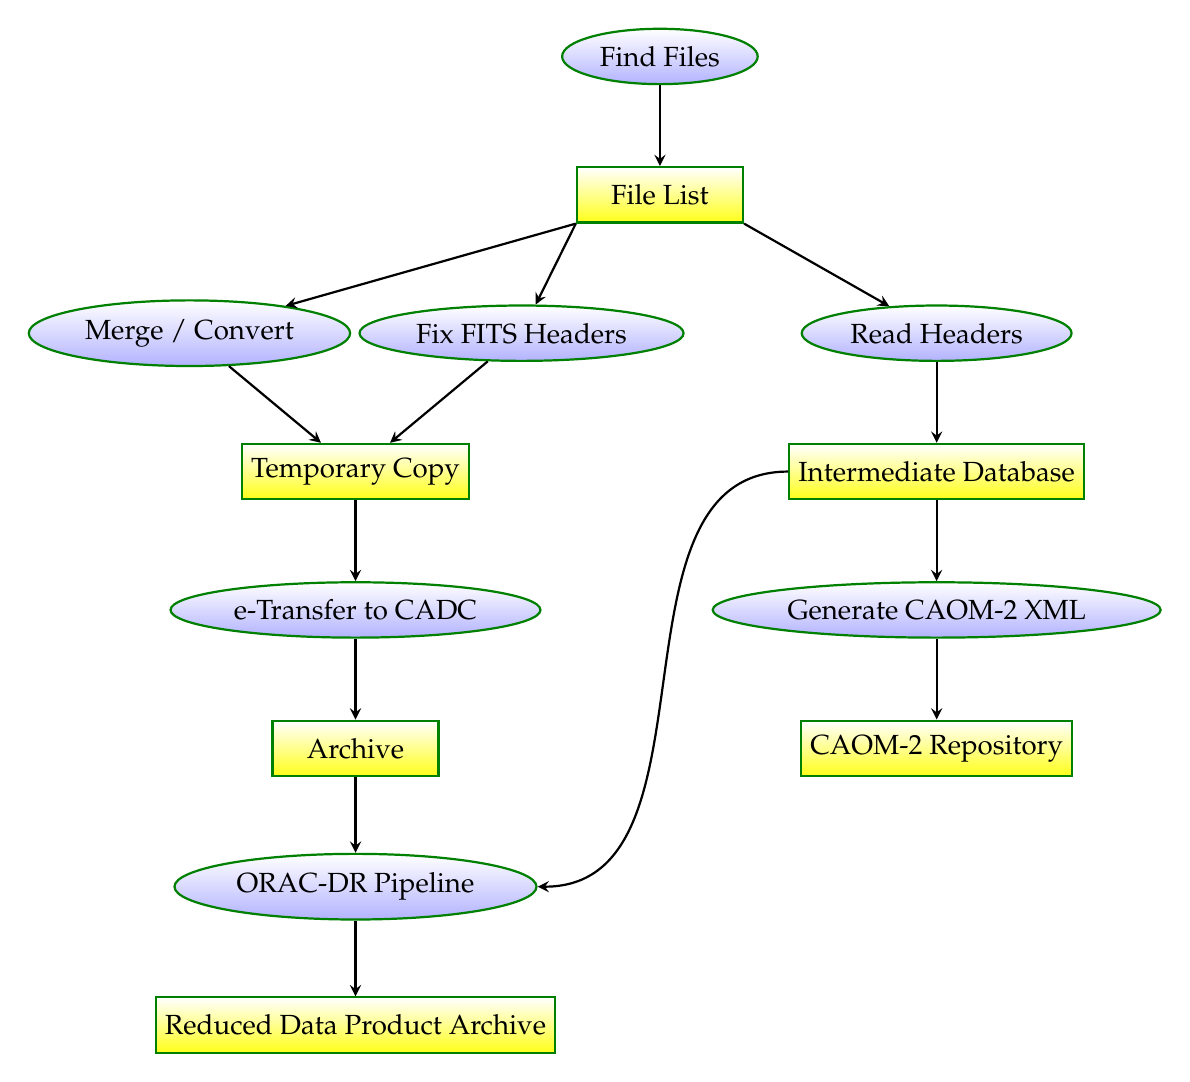
\begin{tikzpicture} [node distance=5em, every edge/.style={link, stealth-}]

% Finding Files

\node[action] (find) [] {Find Files};

\node[data] (list) [below of=find] {File List} edge (find);

% E-transfer

\node[action] (fixfits) [below of=list, xshift=-5em] {Fix FITS Headers} edge (list.south west);

\node[action] (convertobs) [below of=list, xshift=-17em] {Merge / Convert} edge (list.south west);

\node[data] (tempfiles) [below of=fixfits, xshift=-6em] {Temporary Copy} edge (fixfits) edge(convertobs);

\node[action] (etransfer) [below of=tempfiles] {e-Transfer to CADC} edge (tempfiles);

\node[data] (filearchive) [below of=etransfer] {Archive} edge (etransfer);


% Headers and Ingestion

\node[action] (readhead) [below of=list, xshift=10em] {Read Headers} edge (list.south east);

\node[data] (database) [below of=readhead] {Intermediate Database} edge (readhead);

\node[action] (caom2xml) [below of=database] {Generate CAOM-2 XML} edge (database);

\node[data] (metaarchive) [below of=caom2xml] {CAOM-2 Repository} edge (caom2xml);

% Pipeline

\node[action] (pipeline) [below of=filearchive] {ORAC-DR Pipeline} edge (filearchive) edge [in=180,out=0] (database.west);

\node[data] (product) [below of=pipeline] {Reduced Data Product Archive} edge (pipeline);

\end{tikzpicture}



\end{document}
